%!TEX root=paper/paper.tex
\section{Method}\label{sec:det_method}

%!TEX root=paper/paper.tex
\subsection{MDP Formulation}\label{sec:mdp_formulation}

To model the \textbf{action selection} policy $\pi(x): \mathcal{X} \mapsto 2^\mathcal{A}$, we introduce the Markov Decision Process (MDP), which defines a single \emph{episode} of selecting actions for some instance $x$.

\begin{mydef} \label{def:MDP}
The \textbf{feature selection MDP} consists of the tuple $(\mathcal{S}, \mathcal{A}, T(\cdot), R(\cdot), \gamma)$:

\begin{itemize}
\item \textbf{State} $s \in \mathcal{S}$ stores the selected action subset $\mathcal{A}_{\pi(x)}$, resulting observations, and total cost $C_{\mathcal{A}_{\pi(x)}}$.
\item The set of \textbf{actions} $\mathcal{A}$.
\item The \textbf{state transition} distribution $T(s' \mid s, a)$ can depend on the instance $x$.
\item The \textbf{reward} function $R(s, a, s') \mapsto \mathbb{R}$ is manually specified, and depends on the actions taken and the instance $x$.
\item The discount $\gamma$ determines amount of \textbf{lookahead} in selecting actions: if 0, actions are selected greedily based on their immediate reward; if 1, the reward accrued by subsequent actions is given just as much weight as the reward of the current action.
\end{itemize}
\end{mydef}

\PM{Trajectories and reward}
A recognition \emph{episode} takes an image $\mathcal{I}$ and proceeds from the initial state $s^0$ and action $a^0$ to the next pair $(s^1,a^1)$, and so on until $(s^J,a^J)$, where $J$ is the last step of the process with $t \le T_d$.
At that point, the policy is terminated, and a new episode can begin on a new image.
We call this a \emph{trajectory} $\xi = (s_0, a_0, s_1, r_1, \dots, a_{I-1}, s_I, r_I)$, where $I$ is the total number of actions taken (and therefore features selected), $s_0$ is the initial state, $a_i \sim \pi(a \mid s_i)$ is chosen by the \emph{policy} $\pi(a \mid s)$, and $s_{i+1} \sim T(s \mid s_i, a_i)$, which can depend on $x$.
The total expected reward (value) of an MDP episode is written as
\begin{equation}\label{eq:expected_reward}
V_\pi(s_0) =
\mathbb{E}_{\xi \sim \left\{ \pi, x \right\}} r(\xi) =
\mathbb{E}_{\xi \sim \left\{ \pi, x \right\}} \left[ \sum_{i=0}^I \gamma^i \, r_i \right]
\end{equation}

\PM{Q-Value function}
We seek $\pi$ that maximizes \autoref{eq:expected_reward}.
If we had a function accurately predicting the value of taking an action in a state, we could define the policy as simply taking the action with maximum value from any state.
We specify this function $Q(s,a): S \times \mathcal{A} \mapsto \mathbb{R}$, where $S$ is the space of all possible states, to assign a value to a potential action $a \in \mathcal{A}$ given the current state $s$ of the decision process.
We can then define the policy $\pi$ as simply $\argmax_{a_i \in \mathcal{A} \setminus \mathcal{O}} Q(s,a_i)$.
The Q-function is defined and learned recursively:
\begin{align}\label{eq:recursive_value}
Q^\pi(s^j,a) = \mathbb{E}_{s^{j+1}} [R(s^j,a) + \gamma Q^\pi(s^{j+1},\pi(s^{j+1}))]
\end{align}

\subsection{Learning the policy}
\PM{Function approximation}
Although the action space $\mathcal{A}$ is manageable, the space of possible states $S$ is intractable, and we must use function approximation to represent $Q(s,a)$: a common technique in reinforcement learning \parencite{Sutton1998}.
We featurize the state-action pair and assume linear structure:
\begin{align}\label{eq:policy}
Q^\pi(s,a) = \theta_\pi^\top \phi(s,a)
\end{align}
where $\phi: \mathcal{S} \times \mathcal{A} \mapsto \mathbb{R}^{d_s}$ is the state featurization function, $d_s$ is the dimensionality of the state feature vector, and $\theta^\pi$ is a vector of weights that defines the policy $\pi$.

\PM{Policy function}
Specifically, the policy is defined as
\begin{equation}
\pi(a \mid s) = \frac{1}{Z} \exp\left(\frac{1}{\tau} \theta^T \phi(s, a)\right)
\end{equation}
where $Z$ is the appropriate normalization and $\tau$ is a temperature parameter that controls the level of exploration vs. exploitation in the policy.
As $\tau \rightarrow 0$, ${\pi(a \mid s)}$ becomes highly peaked at $\argmax_a Q(s,a)$; it becomes uniform as $\tau \rightarrow \infty$.
In training, this parameter is turned down gradually.

\begin{figure}[ht]
\centering
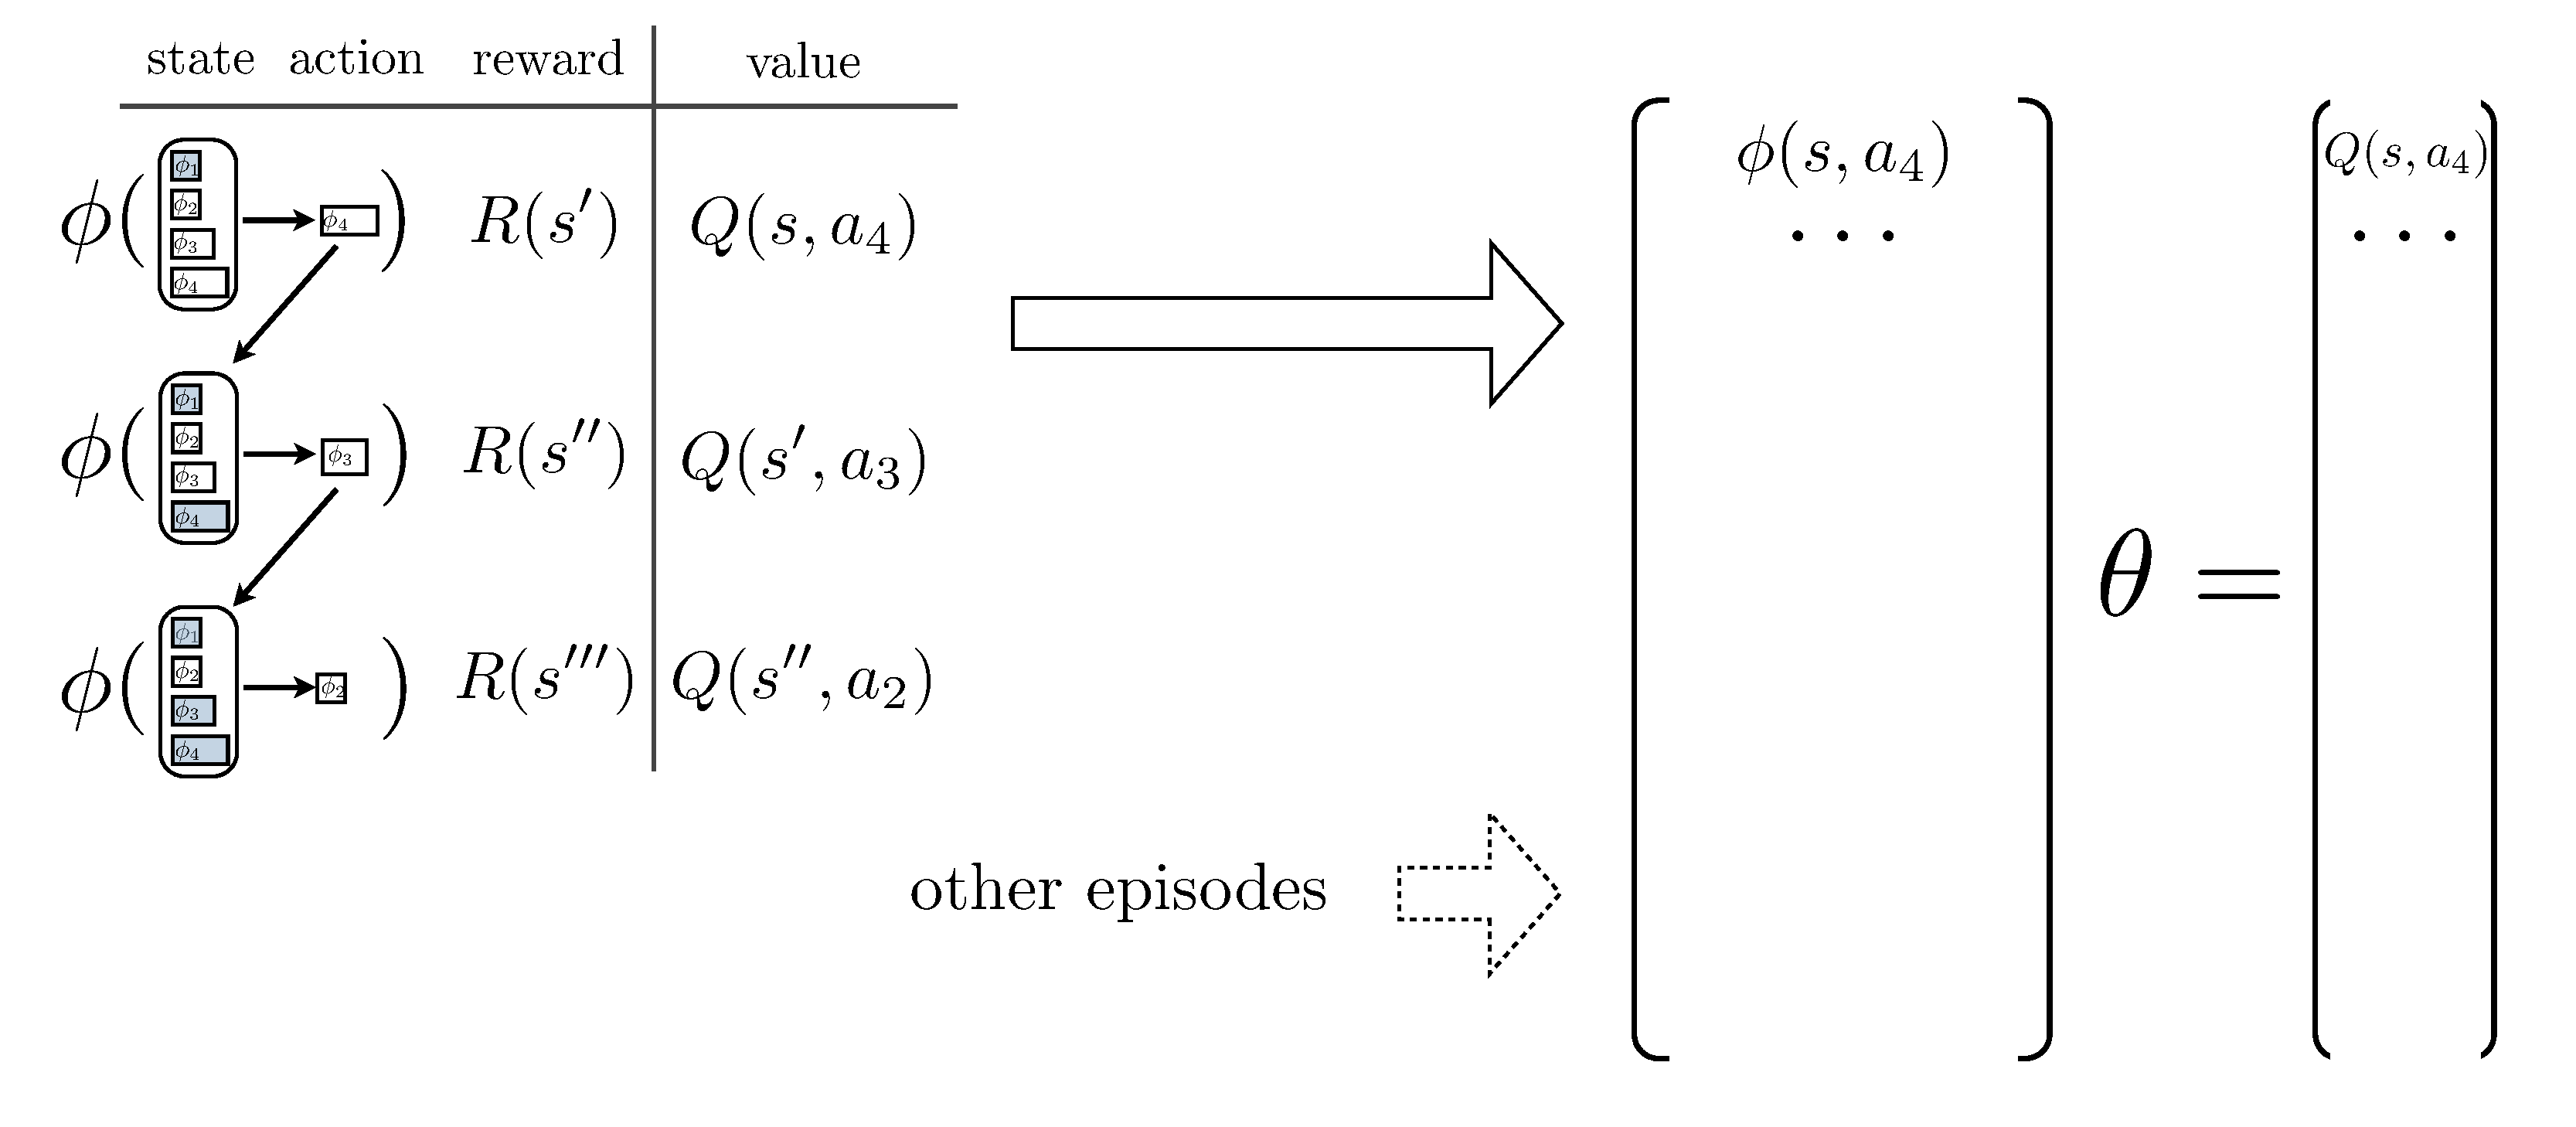
\includegraphics[width=\linewidth]{../../figures/qiteration_explanation.pdf}
\caption[
Explanation of the Q-iteration method.]{
We sample $Q^\pi(s, a) = \mathbb{E}_{s'} \left[ R(s') + \gamma Q^\pi(s', \pi(s')) \right] = \theta^T \phi(s, a)$ by running the policy over many images.
Once an episode is complete, the $Q$-value at each $(s, a)$ can be determined.
To update the policy, simply minimize the prediction error of $\theta$, and repeat.
\label{fig:qiteration_explanation}}
\end{figure}


\PM{Sampling Q-function}
While we can't directly compute the expectation in \autoref{eq:recursive_value}, we can sample it by running actual episodes to gather $<s,a,r,s'>$ samples, where $r$ is the reward obtained by taking action $a$ in state $s$, and $s'$ is the following state.
We then learn the optimal policy by repeatedly gathering samples with the current policy, minimizing the error between the discounted reward to the end of the episode as predicted by our current $Q(s^j,a)$ and the actual values gathered, and updating the policy with the resulting weights.
This method is akin to fitted Q-iteration, a variant of generalized policy iteration \parencite{Ernst2005,Sutton1998}.
\autoref{fig:qiteration_explanation} shows a step of this process.

\PM{Gathering trajectories}
During training, we gather samples starting from either a random feasible state, with probability $\epsilon$, or from the initial empty state otherwise.
Both $\epsilon$ and $\tau$ parameters decay exponentially with the number of training iterations.
Training is terminated if $\pi_{\theta_{i+1}}$ returns the exact same sequence of episodes $\xi$ on a validation set as $\pi_{\theta_{i}}$.
During test time, $\epsilon$ is set to $0.05$.

\PM{Block-coding}
To formulate learning the policy as a single regression problem, we could represent the features in block form, where $\phi(s,a)$ is a vector of size $F|\mathcal{A}|$, with all values set to $0$ except for the $F$-sized block corresponding to $a$.
An implementation detail: instead of block-coding $\phi(s,a)$, we learn $F$ separate $\theta_f$'s for the features $\phi(s)$: one for each action $a$
To prevent overfitting, we use $L_2$-regularized regression.
The weight $\alpha$ of the regularization term is tied across the $F$ separate regressions and is tuned by cross-validation on 3 folds.

\PM{Details}
We run $15$ iterations of accumulating samples by running $350$ episodes, starting with a baseline policy which will be described in \autoref{sec:det_evaluation}, and cross-validating the regularization parameter at each iteration.
Samples are not thrown away between iterations.

\subsubsection{Greedy vs non-myopic}

\PM{Greedy}
Note from \autoref{eq:recursive_value} that the $\gamma \in [0,1]$ parameter of the MDP controls the level of \emph{discounting} of rewards of future action in computing the value \autoref{eq:expected_reward}.
In the baseline \textbf{greedy} setting, with $\gamma=0$, rewards gained by future actions are not counted at all in determining the value of the current action.
The value function is determined entirely by the immediate reward, and so only completely greedy policies can be learned in this case.
This setting is used as baseline.

\PM{Non-myopic}
In the \textbf{non-myopic} setting, with $\gamma=1$, rewards gained by future actions are valued exactly as much as reward gained by the current action in determining its value.
However, a slightly lower value of $\gamma$ mitigates the effects of increasing uncertainty regarding the state transitions over long episodes.
We set this meta-parameter of our approach through cross-validation, and find that a mid-level value ($0.4$) works best.


%!TEX root=paper/thesis.tex
\subsection{Reward definition}\label{sec:det_reward}

The policy's performance at time $t$ is determined by all detections that are part of the set of observations $\mathbf{o}^j$ at the last state $s^j$ before $t$.
Recall that detector actions returns lists of detection hypotheses.
Therefore, the final AP vs. Time evaluation of an episode is a function $eval(h,T_s,T_d)$ of the history of execution $h=s^0,s^1,\dots,s^J$.
It is precisely the normalized area under the AP vs. Time curve between $T_s$ and $T_d$, as determined by the detections in $\mathbf{o}^j$ for all steps $j$ in the episode.

\begin{figure}[h!]
\centering
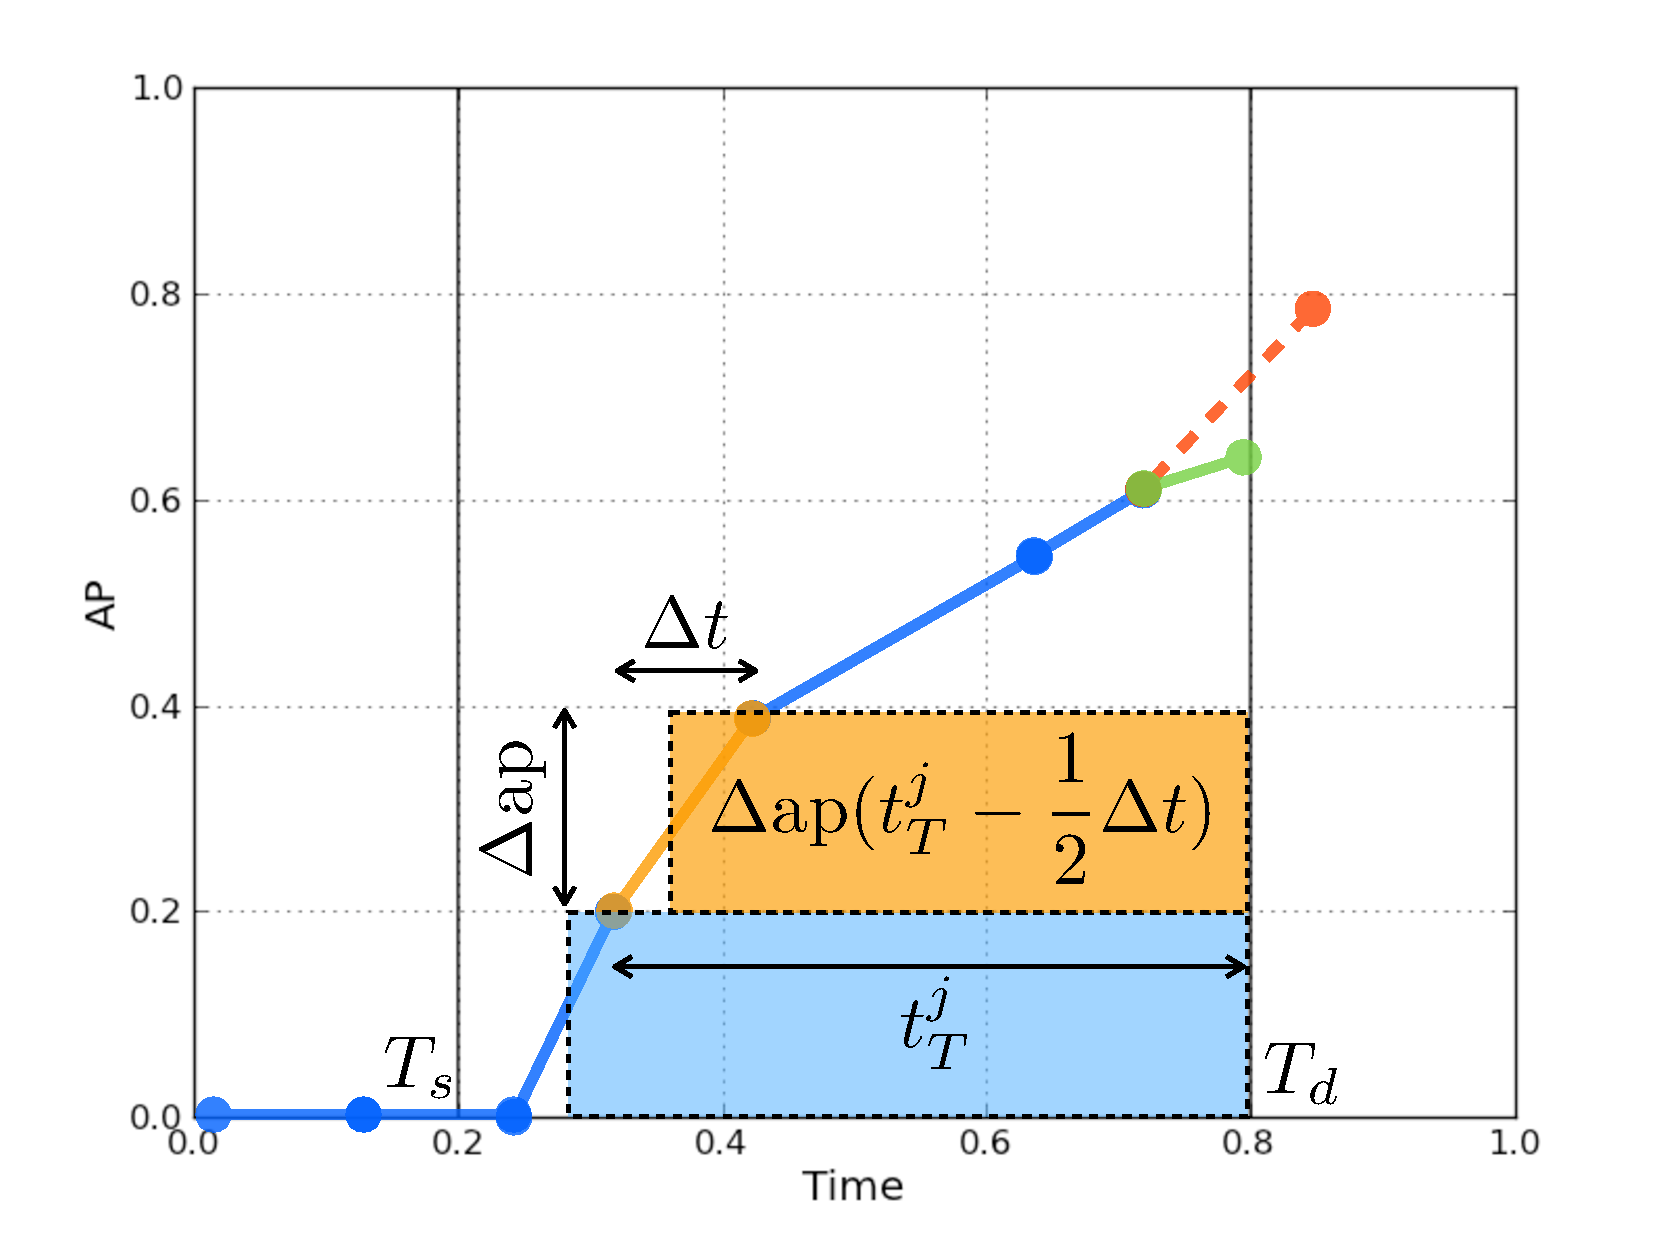
\includegraphics[width=\linewidth]{../../../2011-2012/figures/apvst_expl.pdf}
\caption{
Graphically representing our reward function.
}\label{fig:det_rewards}
\end{figure}


Note from Figure~\ref{fig:det_rewards} that this evaluation function is additive per action, as each action $a$ generates observations that may raise or lower the mean AP of the results so far ($\Delta ap$) and takes a certain time ($\Delta t$).
We can accordingly represent the final evaluation $eval(h,T_s,T_d)$ in terms of individual action rewards: $\sum_{j=0}^J R(s^j,a^j)$.

Specifically, as shown in Figure~\ref{fig:det_rewards}, we define the \emph{reward} of an action $a$ as
\begin{align}\label{eq:advanced}
R(s^j,a) = \Delta \text{ap} (t_T^j-\frac{1}{2}\Delta t)
\end{align}
where $t_T^j$ is the time left until $T_d$ at state $s^j$, and $\Delta t$ and $\Delta \text{ap}$ are the time taken and AP change produced by the action $a$.
(We do not account for $T_s$ here for clarity of exposition.)

\PM{Summary}
In summary, we learn the $\theta$ by \emph{policy iteration}.
First, we gather $(s, a, r, s')$ samples by running episodes (to completion) with the current policy parameters $\theta_i$.
From these samples, $\hat{Q}(s, a)$ values are computed, and $\theta_{i+1}$ are given by $L_2$-regularized least squares solution to $\hat{Q}(s, a) = \theta^T \phi(s, a)$, on all states that we have seen in training.
With pre-computed detections on the PASCAL VOC 2007 dataset, the training procedure takes about $4$ hours on an $8$-core \emph{Xeon E5620} machine.


%!TEX root=paper/paper.tex
\subsection{Features of the state}\label{sec:det_features}

\PM{Open vs Closed Loop}
An \emph{open-loop} policy, such as the common classifier cascade \cite{Viola2004}, takes actions in a sequence that does not depend on observations received from previous actions.
In contrast, our goal is to learn a dynamic, or \emph{closed-loop}, policy, which would exploit the signal in scene and inter-object context for a maximally efficient path through the actions.

\PM{State}
We refer to the information available to the decision process as the \emph{state} $s$.
The state includes the current estimate of the distribution over class presence variables $P(\mathbf{C}) = \{P(C_0), \ldots, P(C_K)\}$, where we write $P(C_k)$ to mean $P(C_k=1)$ (class $k$ is present in the image).
Additionally, the state records that an action $a_i$ has been taken by adding it to the initially empty set $\mathcal{O}$ and recording the resulting observations $o_i$.
We refer to the current set of observations as $\mathbf{o} = \{o_i | a_i \in \mathcal{O}\}$.
The state also keeps track of the time into episode $t$, and the setup and deadline times $T_s,T_d$.

\PM{Dynamic features}
Our policy is at its base determined by a linear function of the features of the state:
\begin{align}
\pi(s) = \argmax_{a_i \in \mathcal{A} \setminus \mathcal{O}} \theta_\pi^\top \phi(s,a_i).
\end{align}
Since we want to be able to learn a dynamic policy, the observations $\mathbf{o}$ that are part of the state $s$ should play a role in determining the value of a potential action.

We include the following quantities as features $\phi(s,a)$:

\begin{tabularx}{0.8\linewidth}{p{0.23\linewidth}p{0.69\linewidth}}
$P(C_a)$ & The prior probability of the class that corresponds to the detector of action $a$ (omitted for the scene-context action).\\
$P(C_0|\mathbf{o}) \ldots P(C_K|\mathbf{o})$ & The probabilities for all classes, conditioned on the current set of observations.\\
$H(C_0|\mathbf{o}) \ldots H(C_K|\mathbf{o})$ & The entropies for all classes, conditioned on the current set of observations. \\
\end{tabularx}

Additionally, we include the mean and maximum of $[H(C_0|\mathbf{o}) \ldots H(C_K|\mathbf{o})]$, and $4$ time features that represent the times until start and deadline, for a total of $F = 1+2K+6$ features.

\PM{Augmented MDP}
We note that this setup is commonly used to solve Markov Decision Processes \cite{Sutton1998}.
There are two related limitations of MDPs when it comes to most systems of interesting complexity, however: the state has to be functionally approximated instead of exhaustively enumerated; and some aspects of the state are not observed, making the problem a Partially Observed MDP (POMDP), for which exact solution methods are intractable for all but rather small problems \cite{Roy2002}.
Our initial solution to the problem of partial observability is to include features corresponding to our level of uncertainty into the feature representation, as in the technique of \emph{augmented} MDPs \cite{Kwok2004}.

\begin{figure}[h!]
\centering
\begin{subfigure}[t]{.8\linewidth}
    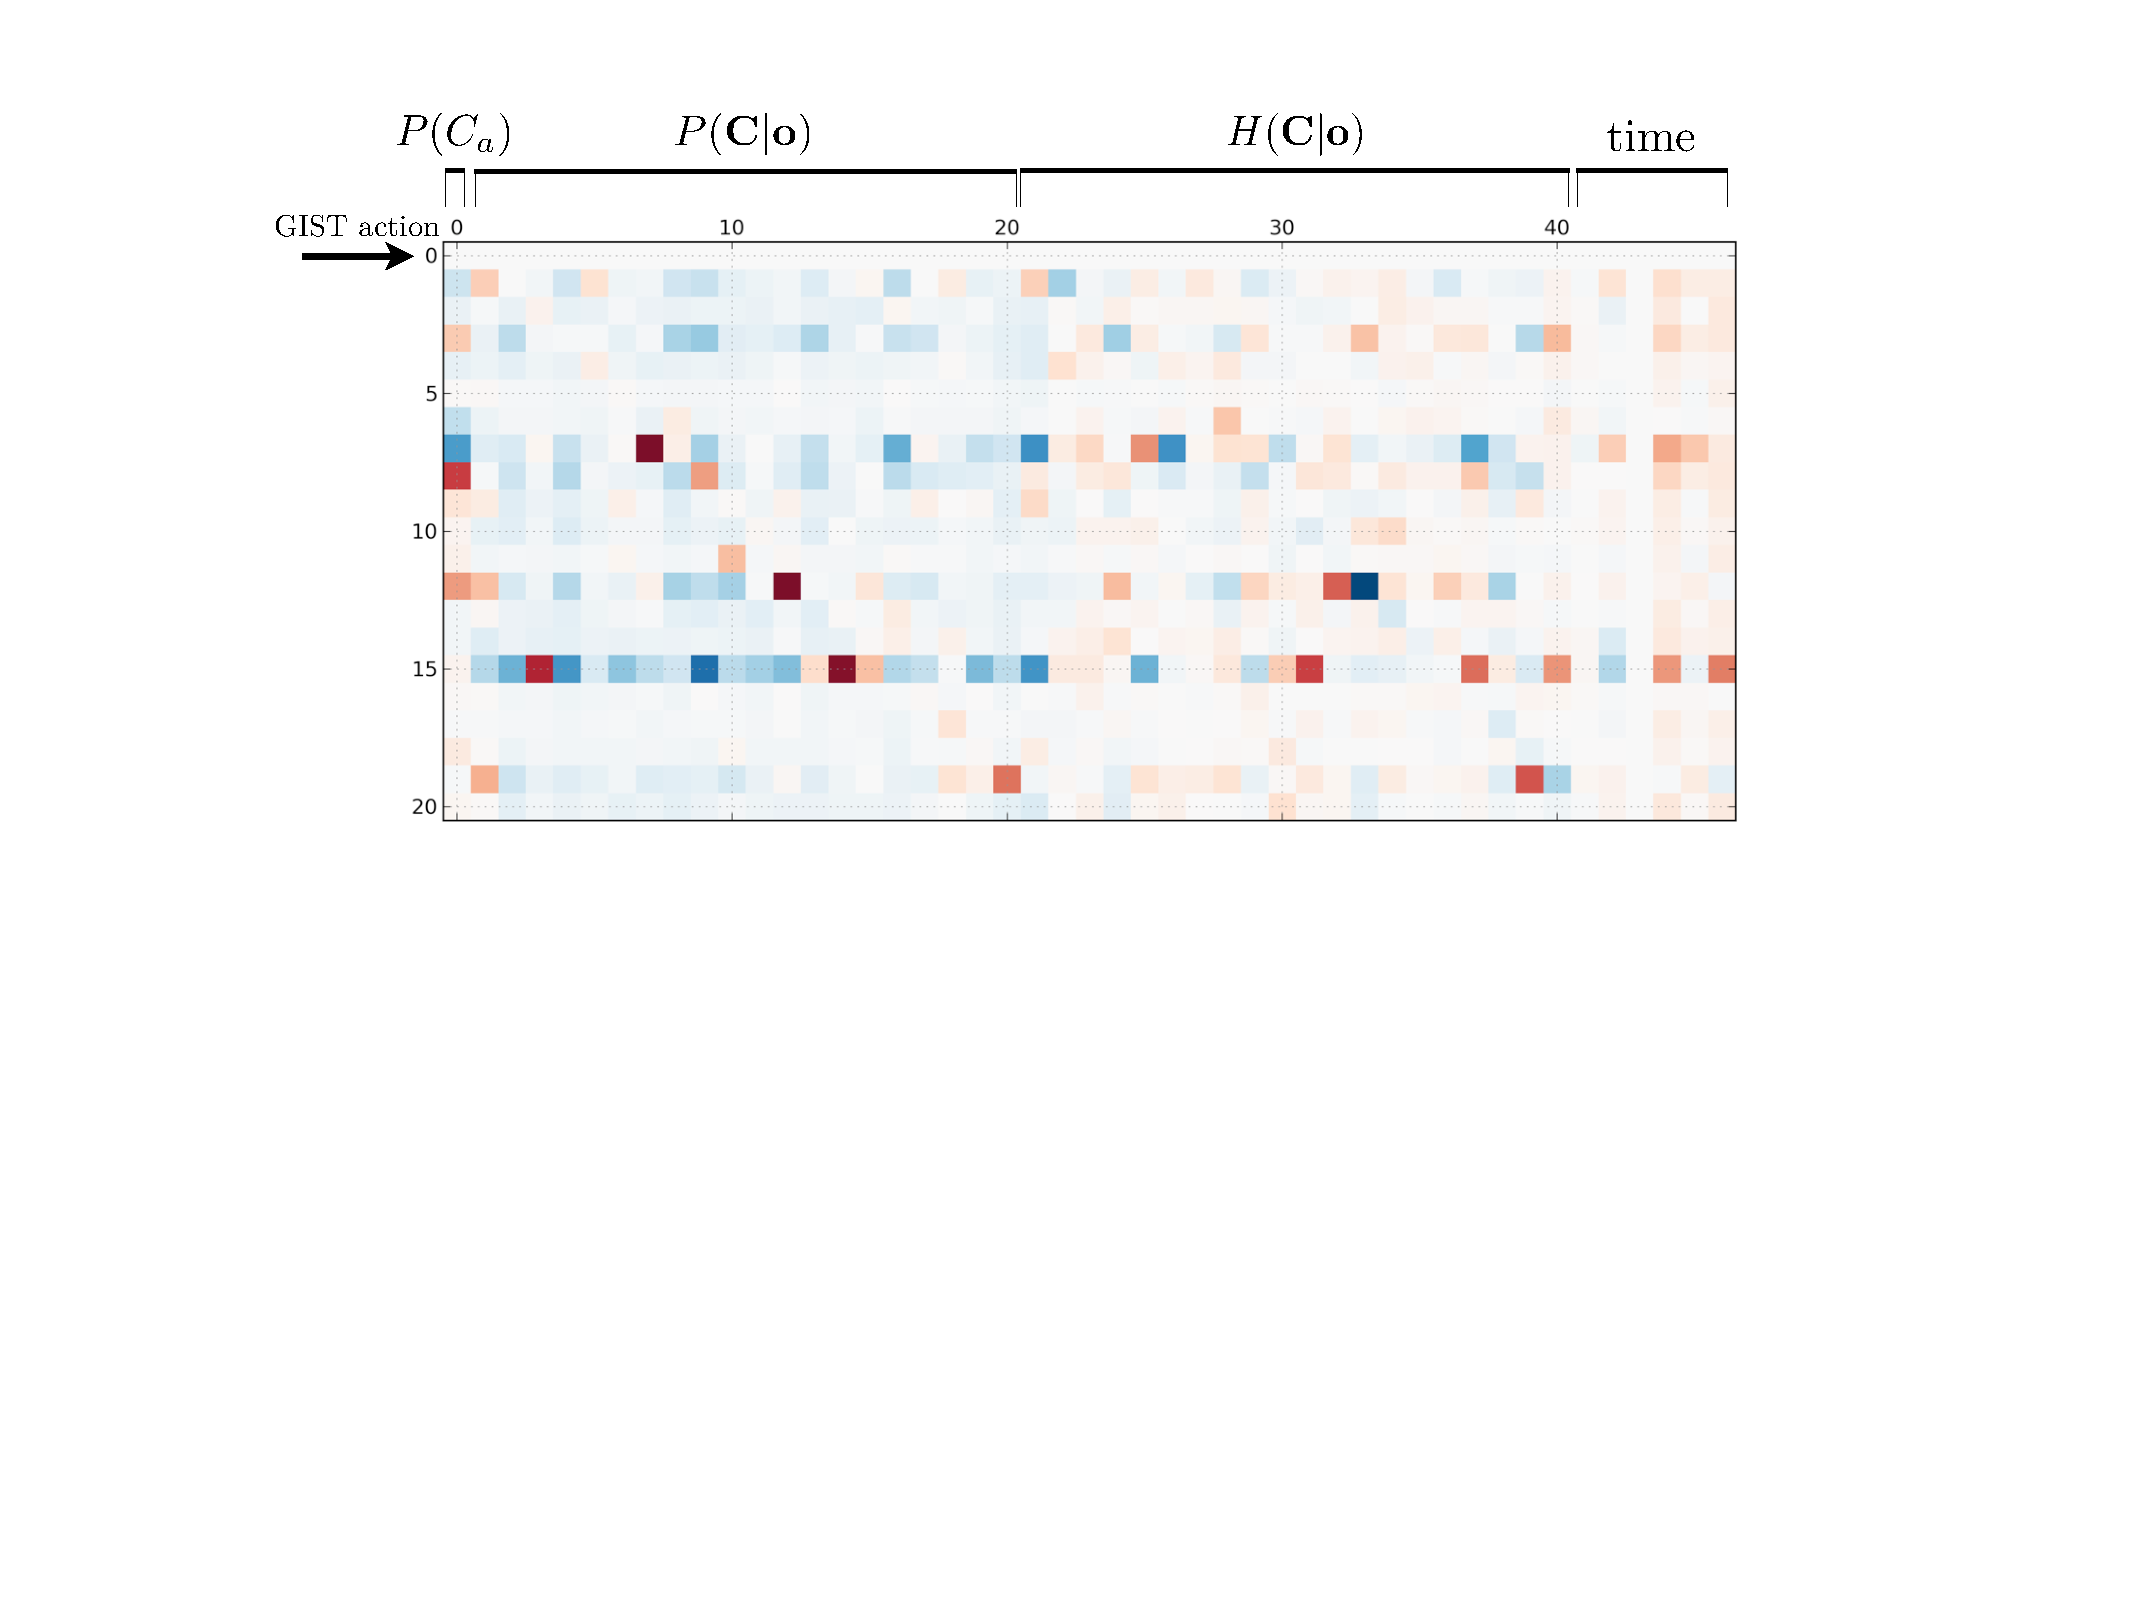
\includegraphics[width=\linewidth]{../../../2011-2012/figures/weights_greedy}
    \caption{Greedy}
\end{subfigure}\\
\begin{subfigure}[t]{.8\linewidth}
    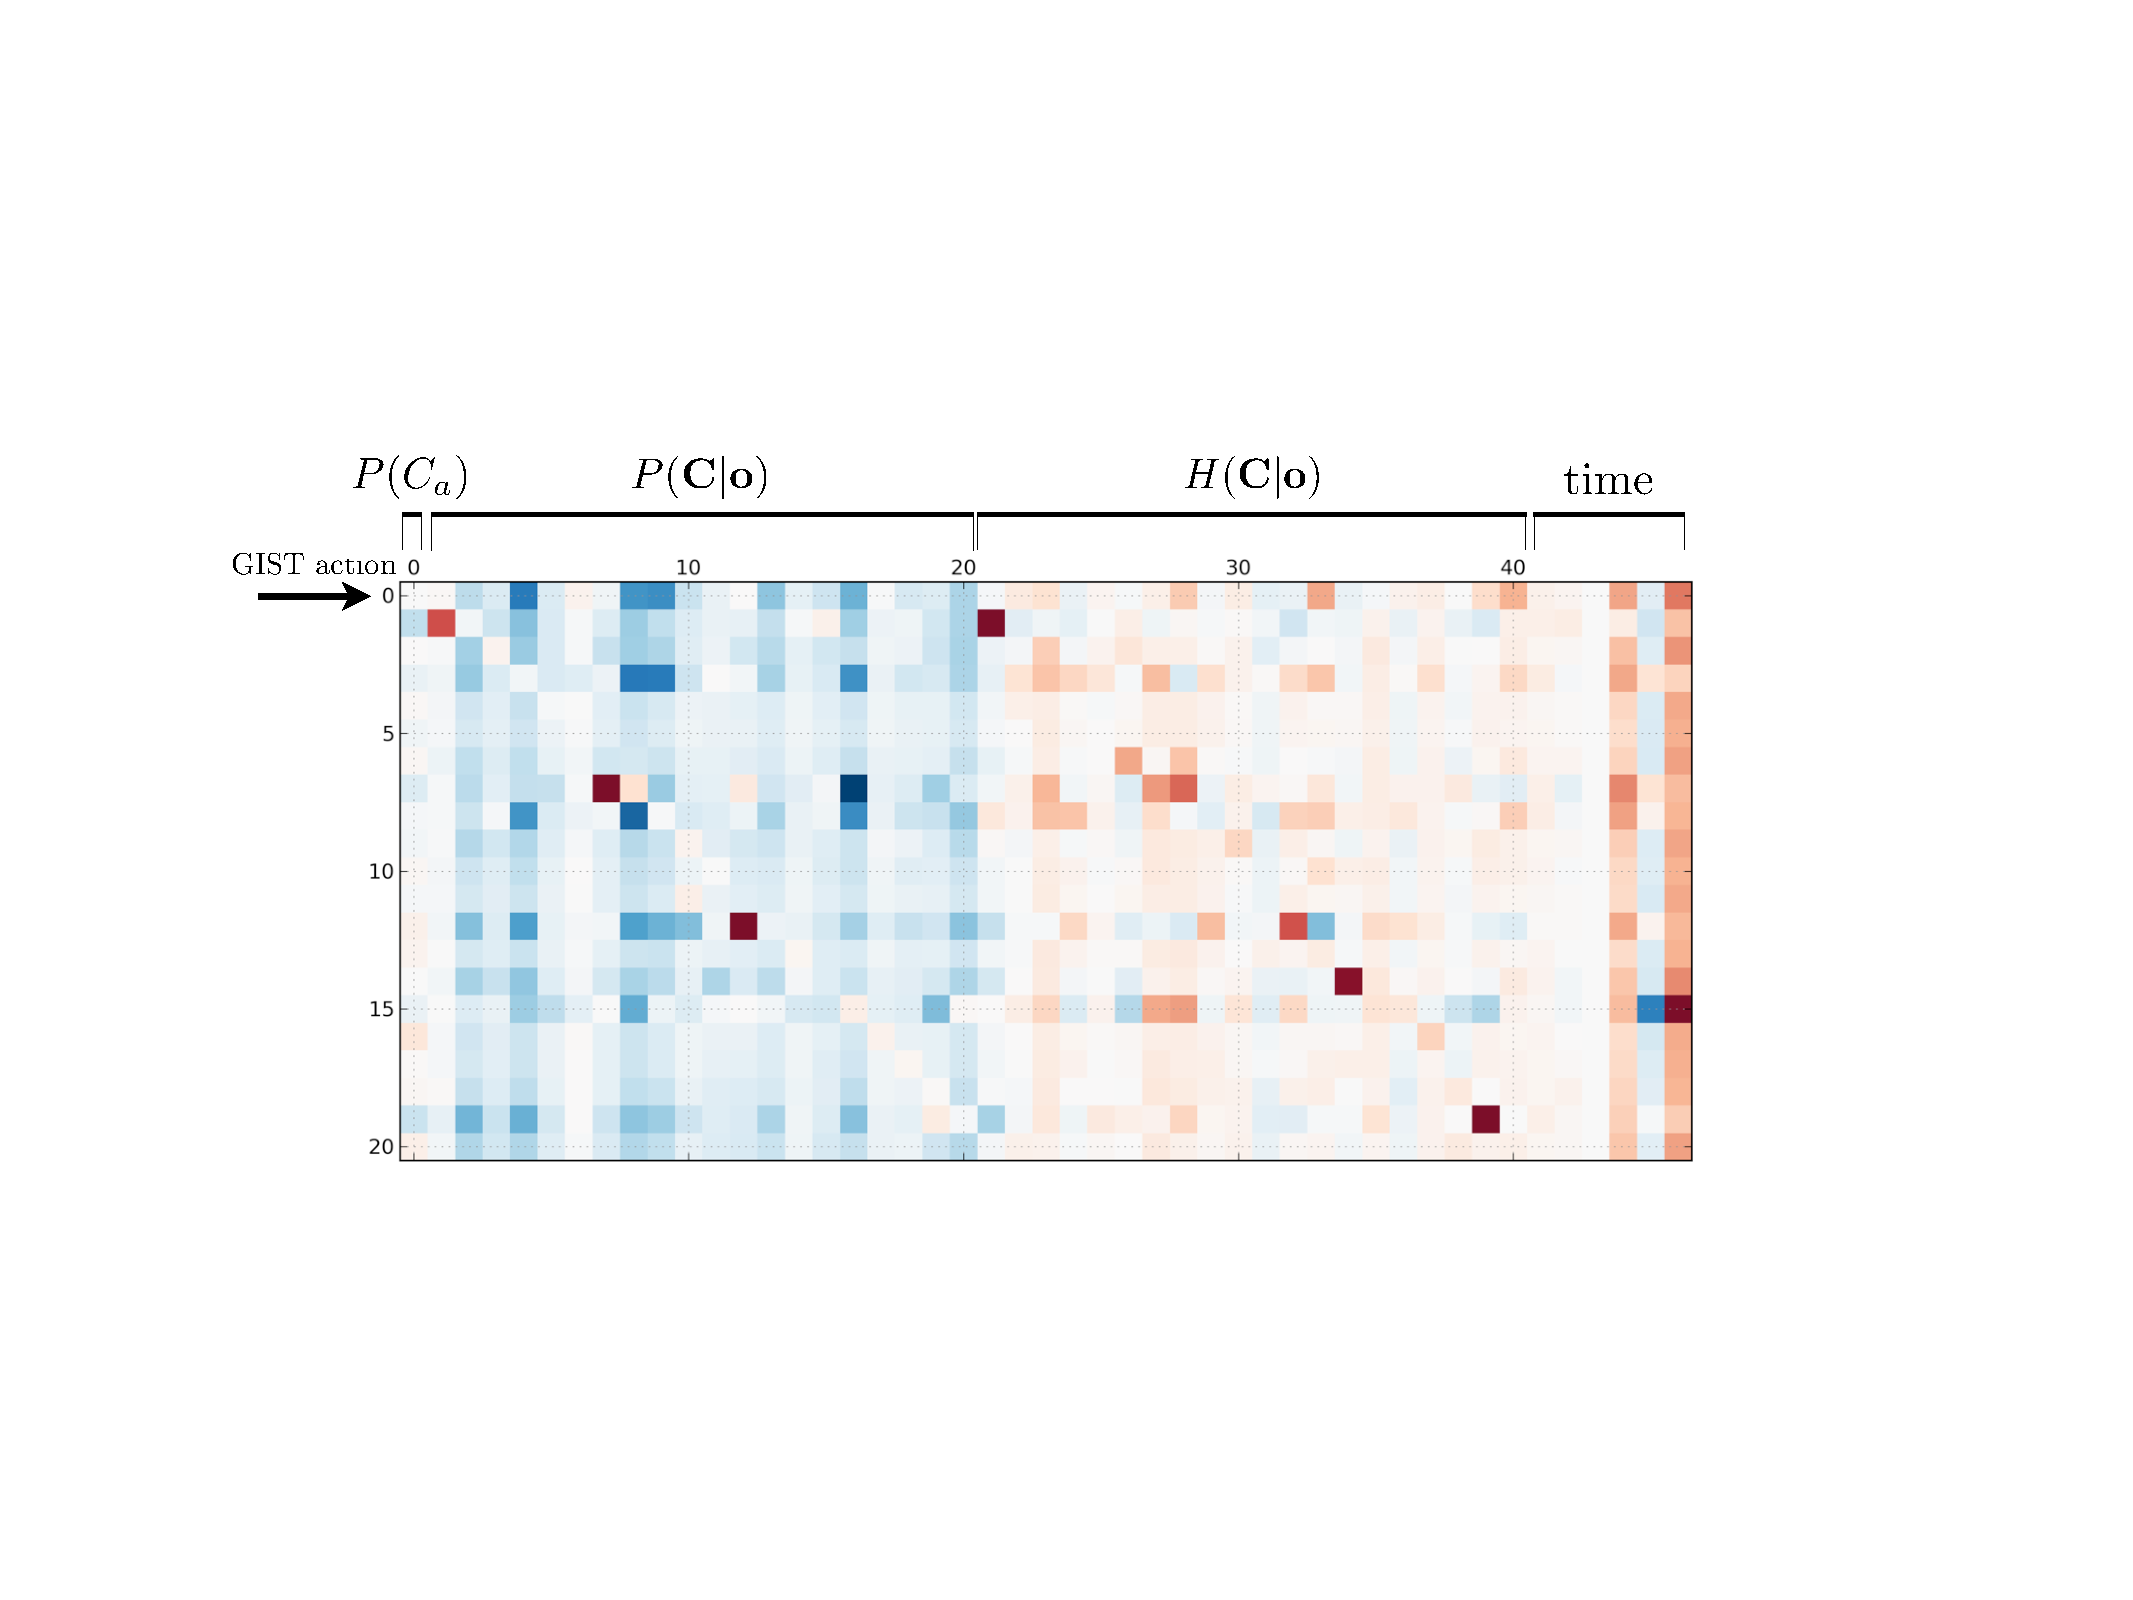
\includegraphics[width=\linewidth]{../../../2011-2012/figures/weights_rl}
    \caption{Reinforcement Learning}
\end{subfigure}
\caption[Learned policy weights for the detection approach.]{
Learned policy weights $\theta_\pi$ (best viewed in color: red corresponds to positive, blue to negative values).
The first row corresponds to the scene-level action, which does not generate detections itself but only helps reduce uncertainty about the contents of the image.
Note that in the greedy learning case, this action is learned to never be taken, but it is shown to be useful in the reinforcement learning case.
}
\label{fig:det_weights}
\end{figure}


\PM{Illustration}
As an illustration, we visualize the learned weights on these features in \autoref{fig:det_weights}, reshaped such that each row shows the weights learned for an action, with the top row representing the scene context action and then next $20$ rows corresponding to the PASCAL VOC class detector actions.
\todo{say something about this}

\subsubsection{Updating with observations}\label{sec:det_features_updating}

\PM{Class correlations}
The bulk of our feature representation is formed by probability of individual class occurrence, conditioned on the observations so far: $P(C_0|\mathbf{o}) \ldots P(C_K|\mathbf{o})$.
This allows the action-value function to learn correlations between presence of different classes, and so the policy can look for the most probable classes given the observations.
However, higher-order co-occurrences are not well represented in this form.
Additionally, updating $P(C_i|\mathbf{o})$ presents choices regarding independence assumptions between the classes.

\PM{Direct vs. MRF update}
We evaluate two approaches for updating probabilities: \emph{direct} and \emph{MRF}.
In the \emph{direct} method, $P(C_i|\mathbf{o}) = score(C_i)$ if $\mathbf{o}$ includes the observations for class $C_i$ and $P(C_i|\mathbf{o}) = P(C_i)$ otherwise.
This means that an observation of class $i$ does not directly influence the estimated probability of any class but $C_i$.
The \emph{MRF} approach employs a pairwise fully-connected Markov Random Field (MRF), as shown in Figure~\ref{fig:figure1}, with the observation nodes set to $score(C_i)$ appropriately, or considered unobserved.

\PM{Learning MRF}
The graphical model structure is set as fully-connected, but some classes almost never co-occurr in our dataset.
Accordingly, the edge weights are learned with $L_1$ regularization, which obtains a sparse structure \cite{Lee2006}.
All parameters of the model are trained on fully-observed data, and Loopy Belief Propagation inference is implemented with an open-source graphical model package \cite{Jaimovich2010}.

\PM{Details}
An implementation detail: $score(C_i)$ for $a_{{det}_i}$ is obtained by training a probabilistic classifier on the list of detections, featurized by the top few confidence scores and the total number of detections.
Similarly, $score(C_i)$ for $a_{gist}$ is obtained by training probabilistic classifiers on the GIST feature, for all classes.


\subsection{Summary}

\begin{figure}[ht]
\centering
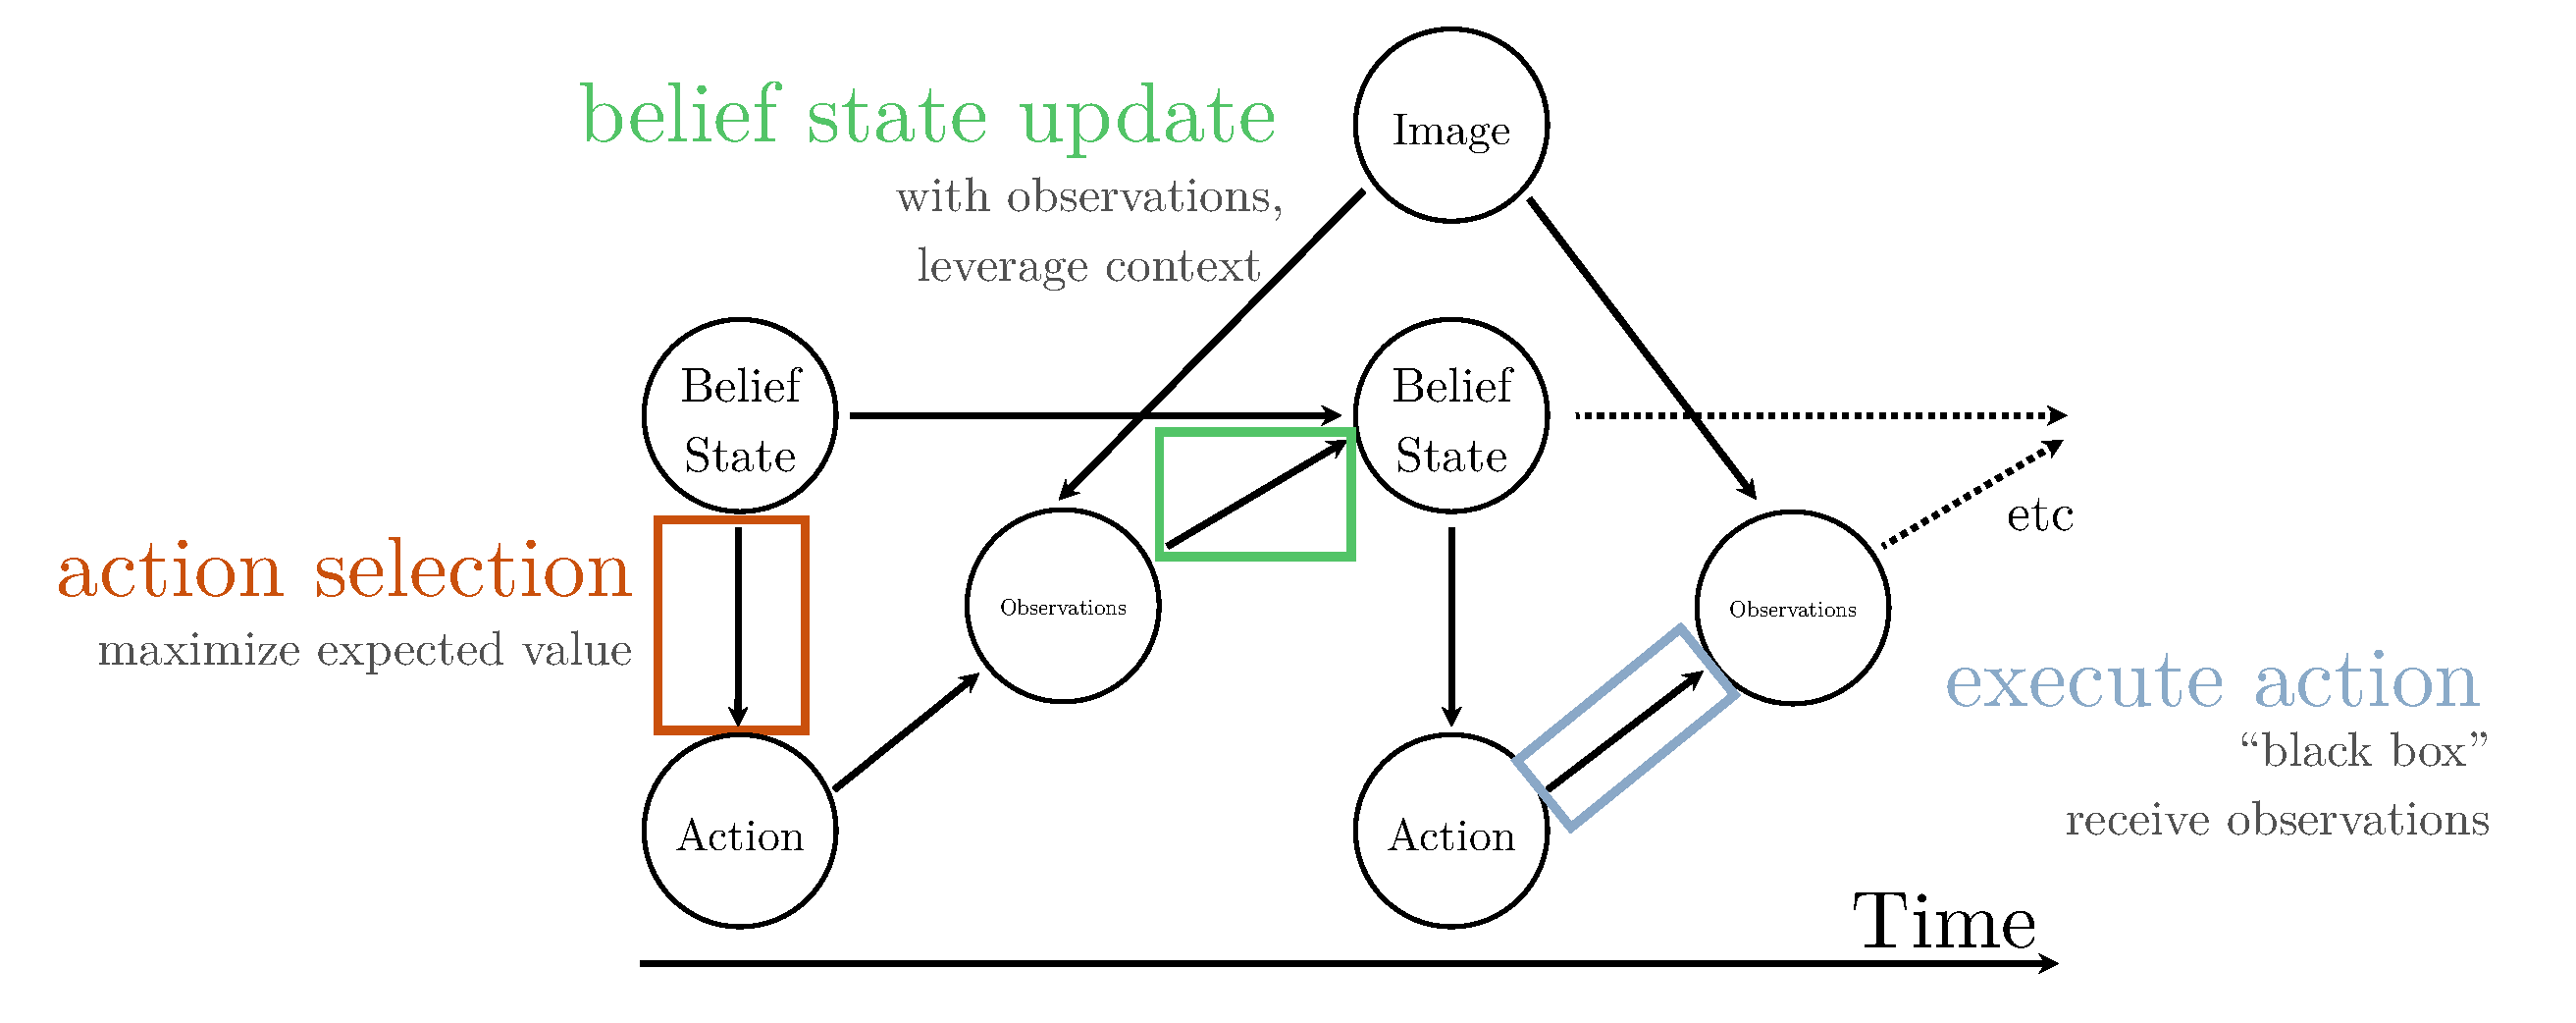
\includegraphics[width=\linewidth]{../../../2011-2012/figures/pomdp_annotated.pdf}
\caption[
Summary of our closed-loop action selection method.]{
Our closed-loop method consists of selecting an action based on the belief state, executing action almost as a ``black box,'' which makes our method very general, and then updating the state with the received observations.
}\label{fig:pomdp_summary}
\end{figure}


Our sequential method is visually summarized in \autoref{fig:pomdp_summary}.
We learn the $\theta$ by \emph{policy iteration}.
First, we gather $(s, a, r, s')$ samples by running episodes (to completion) with the current policy parameters $\theta_i$.
From these samples, $\hat{Q}(s, a)$ values are computed, and $\theta_{i+1}$ are given by $L_2$-regularized least squares solution to $\hat{Q}(s, a) = \theta^T \phi(s, a)$, on all states that we have seen in training.
With pre-computed detections on the PASCAL VOC 2007 dataset, the training procedure takes about $4$ hours on an $8$-core \emph{Xeon E5620} machine.
